%%----------------------------------------------------------------------------------------
\pagestyle{fancy}
%%----------------------------------------------------------------------------------------
%%       PREFAZIONE
%%----------------------------------------------------------------------------------------
\part{Momento statico, baricentro di figure piane}
\section{Introduzione}
\label{paragrafo1-1}
%----------------------------------------------------------------------------------------
\renewcommand{\thefigure}{1~-~1}
\begin{figure}[h]
\centering
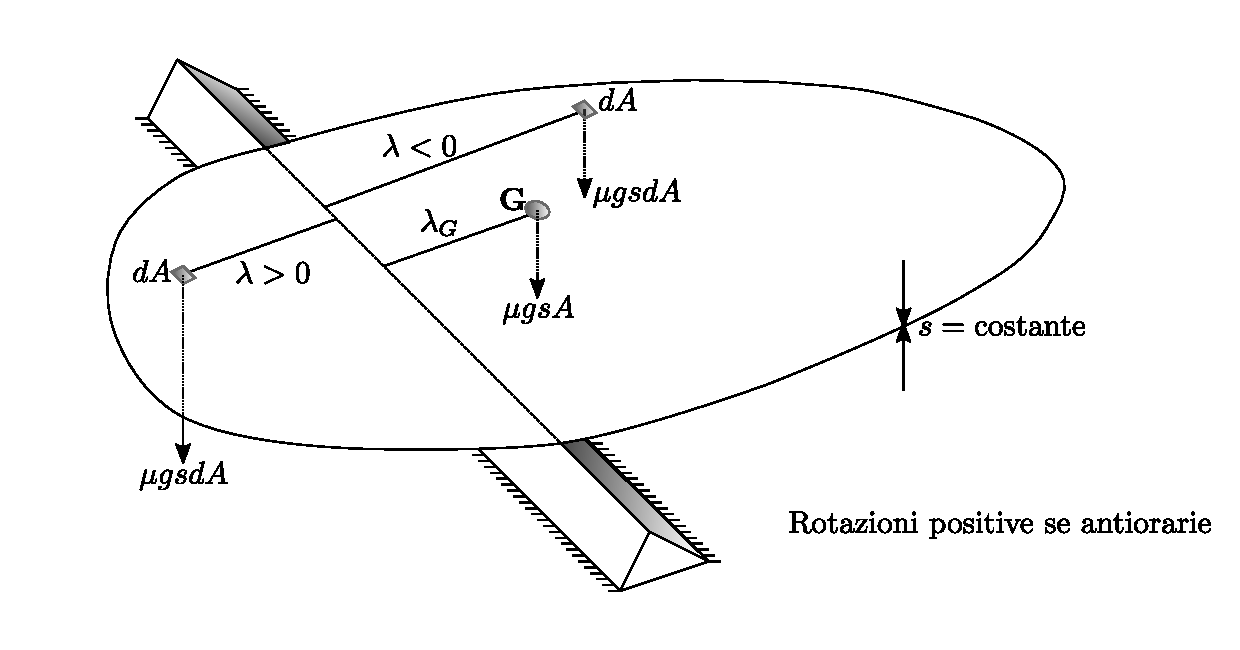
\includegraphics[width=\textwidth]{Immagini/Parte_1/Figura1_1/Figura1_1.pdf}
\caption{}
\label{figura1-1}
\end{figure}
%----------------------------------------------------------------------------------------
\noindent In figura~\ref{figura1-1} è rappresentato un \emph{lamierino} di materiale omogeneo, perfettamente piano, di spessore costante $s$; diciamo $A$ la sua area \emph{in pianta}. Esso è appoggiato su di una linea $r$ perfettamente orizzontale.
%----------------------------------------------------------------------------------------

\noindent La domanda sorge spontanea: il lamierino resterà in equilibrio oppure si ribalterà?
%----------------------------------------------------------------------------------------

\noindent Nel caso della figura la risposta è immediata: esso si ribalterà ruotando intorno alla retta $r$ in senso negativo (in figura si è assunto come verso positivo della rotazione intorno all'asse $r$ quello antiorario).
%----------------------------------------------------------------------------------------

\noindent Vogliamo approfondire, dal punto di vista fisico e matematico il tema in esame. Ogni \emph{pezzettino} di volume $d\mathcal{V}=sdA$ del lamierino ha una massa pari a 
%----------------------------------------------------------------------------------------
\begin{equation*}
dm = \mu sdA
\end{equation*}
%----------------------------------------------------------------------------------------
essendo $\mu$ la \textbf{densità} del materiale.
%----------------------------------------------------------------------------------------

\noindent In presenza di un campo gravitazionale (terrestre o no) su ogni \emph{pezzettino} agirà una forza gravitazionale diretta verso il basso pari 
%----------------------------------------------------------------------------------------
\begin{equation*}
\mu gsdA,
\end{equation*}
%----------------------------------------------------------------------------------------
essendo $g$ l'accelerazione di gravità (che sulla Terra vale $9.81\,\textup{m}/\textup{s}^2$). Ognuna delle suddette forze elementari ha un braccio $\lambda$ rispetto alla retta $r$ e, conseguentemente, ha un momento rispetto ad $r$ pari a 
%----------------------------------------------------------------------------------------
\begin{equation*}
\lambda \mu gsdA.
\end{equation*}
%----------------------------------------------------------------------------------------
\noindent Le forze che stanno a sinistra di $r$ hanno chiaramente un momento positivo (giacché esso promuove una rotazione positiva); ovviamente le forze che stanno a destra di $r$ hanno momento negativo. Si conviene pertanto di attribuire segno positivo alle distanze $\lambda$ delle areole a sinistra di $r$ (e di conseguenza segno negativo a quelle a destra di $r$). 
%----------------------------------------------------------------------------------------

\noindent Il momento risultante rispetto ad $r$ di tutte le forze elementari suddette vale pertanto 
%----------------------------------------------------------------------------------------
\begin{equation*}
M_r = \int\int_A \lambda \mu gsdA
\end{equation*}
%----------------------------------------------------------------------------------------

ed essendo $g$, $\mu$ ed $s$ costanti
%----------------------------------------------------------------------------------------
\begin{equation*}
M_r = \mu gs \int\int_A \lambda dA
\end{equation*}
%----------------------------------------------------------------------------------------

\noindent Naturalmente
%--------------------------------------------------------------------------------------------------------------------------------------------------
\begin{figure}[h!] 
\centering
\begin{tikzpicture}[scale=1.2, node distance=4cm,auto]
\node[block](init){Lamierino in equilibrio su $r$}; 
\node[](equal) at (1.70,0) {$=$};
\node[block, right of=init](var){$M_r=0$};
\node[](plus) at (5,0) {$=$};
\node[block, right of=var](var1){$\int\int_A \lambda dA=0$};
\end{tikzpicture}
\label{}
\end{figure}
%--------------------------------------------------------------------------------------------------------------------------------------------------

\noindent Come è noto, la risultante delle forze elementari $\mu gsdA$ è applicata nel \textbf{baricentro} (detto anche \textbf{centro di massa}) $\mathbf{G}$. 
%--------------------------------------------------------------------------------------------------------------------------------------------------

\noindent Detto $\lambda_G$ la distanza (con segno) di $\mathbf{G}$ da $r$, per il \textsc{Teorema di Varignon} risulta:
%--------------------------------------------------------------------------------------------------------------------------------------------------
\begin{figure}[h!] 
\centering
\begin{tikzpicture}[scale=1.2, node distance=4cm,auto]
\node[block](init){Mom. risultante rispetto ad $r$}; 
\node[](equal) at (1.70,0) {$=$};
\node[block, right of=init](var){Mom. della risultante rispetto ad $r$};
\end{tikzpicture}
\label{}
\end{figure}
%--------------------------------------------------------------------------------------------------------------------------------------------------

\noindent e pertanto 
%----------------------------------------------------------------------------------------
\begin{equation*}
M_r = \mu gs \lambda_G
\end{equation*}
%----------------------------------------------------------------------------------------

\noindent ovvero, semplificando 
%----------------------------------------------------------------------------------------
\begin{equation*}
\int\int_A \lambda dA = A \lambda_G
\end{equation*}
%----------------------------------------------------------------------------------------

\noindent e dunque 
%--------------------------------------------------------------------------------------------------------------------------------------------------
\begin{figure}[h!] 
\centering
\begin{tikzpicture}[scale=1.2, node distance=4cm,auto]
\node[block](init){Lamierino in equilibrio su $r$}; 
\node[](equal) at (1.70,0) {$=$};
\node[block, right of=init](var){$\lambda_G=0$};
\node[](plus) at (5,0) {$=$};
\node[block, right of=var](var1){$\mathbf{G}\in r$};
\end{tikzpicture}
\label{}
\end{figure}
%--------------------------------------------------------------------------------------------------------------------------------------------------
\section{La definizione di momento statico}
%----------------------------------------------------------------------------------------
\renewcommand{\thefigure}{1~-~2}
\begin{figure}[ht]
\centering
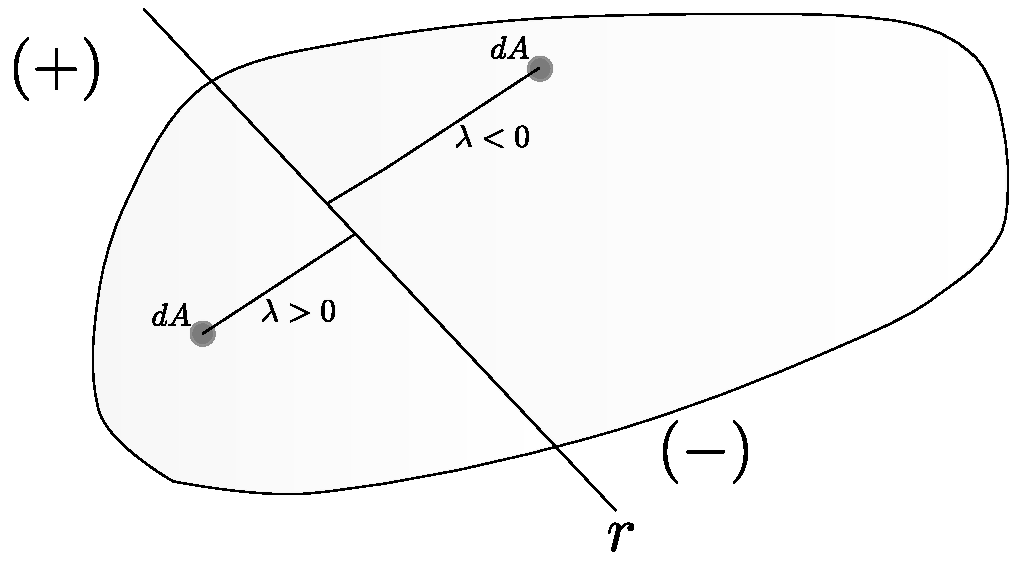
\includegraphics[width=0.55\textwidth]{Immagini/Parte_1/Figura1_2/Figura1_2.pdf}
\caption{}
\label{figura1-2}
\end{figure}
%----------------------------------------------------------------------------------------
\noindent In figura~\ref{figura1-2} è rappresentata una figura piana ed una retta $r$ ad essa complanare. Sia $dA$ una generica areola e $\lambda$ la sua distanza da $r$. Si sono assunte positive le distanze delle areole alla sinistra di $r$ (la scelta è arbitraria). Il prodotto $\lambda dA$ si dice \textbf{momento statico elementare} dell'areola $dA$ rispetto ad $r$. La quantità 
%---------------------------------------------------------------------------------------------------------------------------------------------
\begin{equation} \label{equazione1-1}
\boxed{S_r=\int\int_A \lambda dA}
\tag{1.1}
\end{equation}
%---------------------------------------------------------------------------------------------------------------------------------------------

\noindent si dice \textbf{Momento Statico} della figura rispetto ad $r$. 
%---------------------------------------------------------------------------------------------------------------------------------------------
%----------------------------------------------------------------------------------------
\renewcommand{\thefigure}{1~-~3}
\begin{figure}[h]
\centering
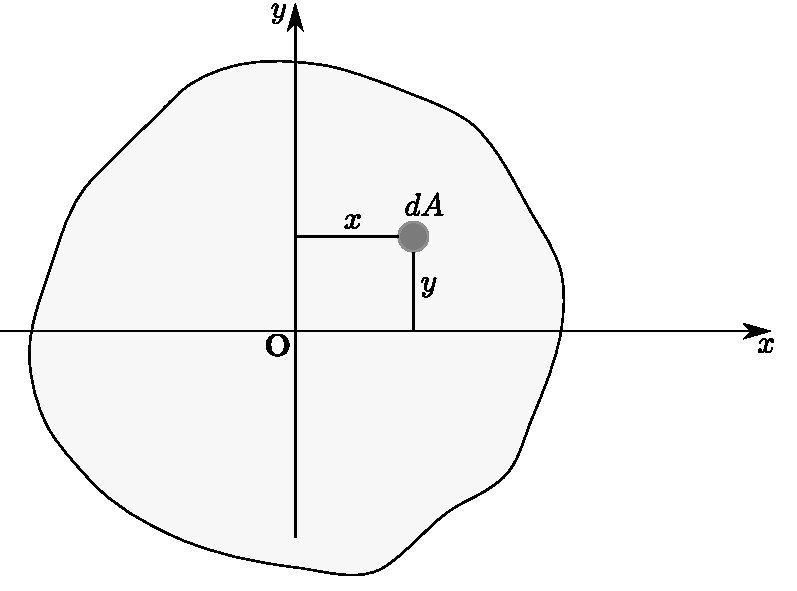
\includegraphics[width=0.5\textwidth]{Immagini/Parte_1/Figura1_3/Figura1_3.pdf}
\caption{}
\label{figura1-3}
\end{figure}
%----------------------------------------------------------------------------------------
\noindent Poiché l'integrale è, in effetti, la somma di tutti i termini elementari $\lambda dA$ presenti nel dominio piano invaso dalla figura, ed essi sono alcuni positivi ed alcuni negativi, si evince dalla~\eqref{equazione1-1} che può essere 
%---------------------------------------------------------------------------------------------------------------------------------------------
\begin{equation*}
\boxed{S_r\, \textup{maggiore, minore o uguale a zero}}
\end{equation*}
%---------------------------------------------------------------------------------------------------------------------------------------------

\noindent Nel caso specifico $S_r < 0$.
%---------------------------------------------------------------------------------------------------------------------------------------------

\noindent Sempre dalla~\eqref{equazione1-1} si evince che il momento statico ha dimensioni
%---------------------------------------------------------------------------------------------------------------------------------------------
\begin{equation*} 
[S_r]=[L]^3
\end{equation*}
%---------------------------------------------------------------------------------------------------------------------------------------------

\noindent e si misura pertanto in $\textup{m}^3$ (o $\textup{cm}^3$ o $\textup{mm}^3$). Il significato fisico di momento statico appare evidente alla luce di quanto detto nel precedente paragrafo: è immediato identificare una figura piana con un lamierino avente $\mu gs = 1$. Nel caso della figura~\ref{figura1-3} la~\eqref{equazione1-1} si particolarizza nelle: 
%---------------------------------------------------------------------------------------------------------------------------------------------
\begin{align} 
\label{equazione1-2}
S_x    &= \int\int_A ydA \tag{1.2a} \\
S_y    &= \int\int_A xdA \tag{1.2b}
\end{align}
%---------------------------------------------------------------------------------------------------------------------------------------------
\section{Baricentro di una figura piana}
%----------------------------------------------------------------------------------------
Per ogni figura piana esiste un punto (ed uno soltanto) che gode della seguente proprietà:
%----------------------------------------------------------------------------------------
%---------------------------------------------------------------------------------------------------------------------------------------------
\begin{equation*} 
\boxed{\textup{Rispetto ad ogni retta passante per esso è nullo il momento statico}}
\end{equation*}
%---------------------------------------------------------------------------------------------------------------------------------------------
Tale punto si dice \textbf{Baricentro} e sarà indicato con $\mathbf{G}$. 
%----------------------------------------------------------------------------------------
È immediato identificare il baricentro di una figura piana con il centro di massa di un lamierino avente la stessa forma in pianta (purché di spessore costante e materiale omogeneo). E allora, in forza di quanto detto al paragrafo~\vref{paragrafo1-1}, possiamo affermare che 
%---------------------------------------------------------------------------------------------------------------------------------------------
\begin{equation} 
\label{equazione1-3}
\boxed{S_r = A\lambda_G}
\tag{1.3}
\end{equation}
%---------------------------------------------------------------------------------------------------------------------------------------------
%----------------------------------------------------------------------------------------
\renewcommand{\thefigure}{1~-~4}
\begin{figure}[h]
\centering
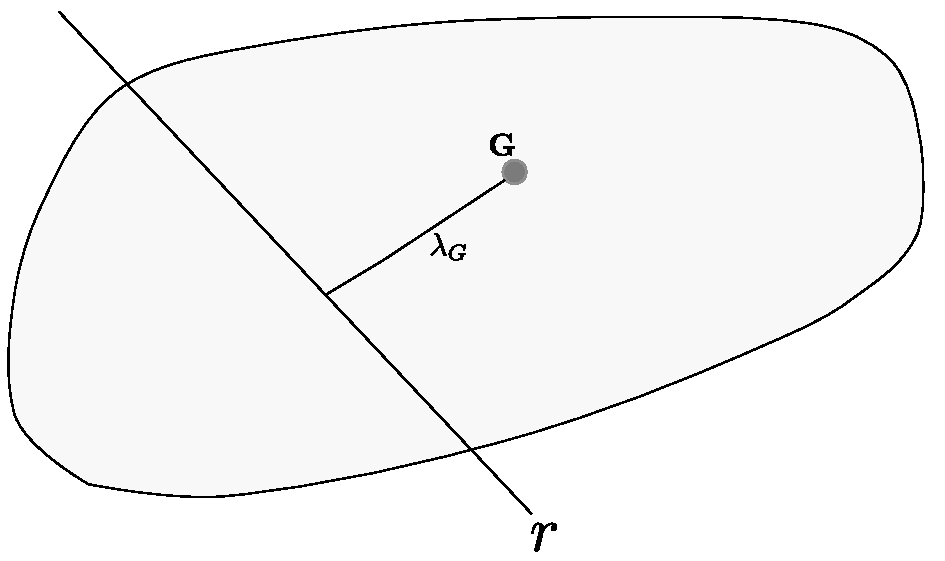
\includegraphics[width=0.5\textwidth]{Immagini/Parte_1/Figura1_4/Figura1_4.pdf}
\caption{}
\label{figura1-4}
\end{figure}
%----------------------------------------------------------------------------------------
La figura~\ref{figura1-4} chiarisce definitivamente quanto appena detto. La~\eqref{equazione1-3} è di notevole importanza: essa consente di calcolare il momento statico $S_r$ senza fare integrali, a patto di conoscere la posizione del baricentro $\mathbf{G}$. 
%----------------------------------------------------------------------------------------

\noindent A questo punto è ovvio che valgono le relazioni 
%---------------------------------------------------------------------------------------------------------------------------------------------
\begin{align} 
S_x    &= Ay_G \tag{1.4a} \label{equazione1-4a} \\
S_y    &= Ax_G \tag{1.4b} \label{equazione1-4b}
\end{align}
%---------------------------------------------------------------------------------------------------------------------------------------------
\renewcommand{\thefigure}{1~-~5}
\begin{figure}[h]
\centering
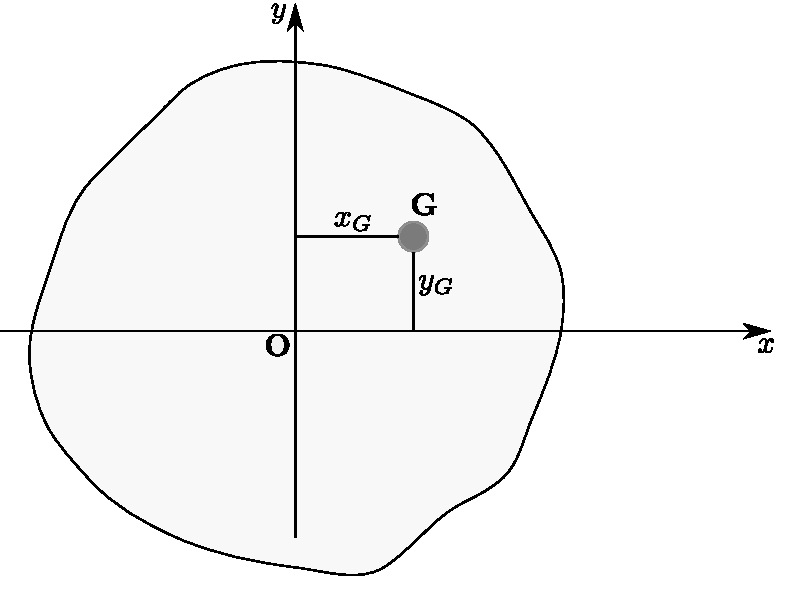
\includegraphics[width=0.5\textwidth]{Immagini/Parte_1/Figura1_5/Figura1_5.pdf}
\caption{}
\label{figura1-5}
\end{figure}
%----------------------------------------------------------------------------------------
%----------------------------------------------------------------------------------------

\noindent Ancora una volta, la figura~\ref{figura1-5} chiarisce quanto appena detto. A proposito di baricentro, si potrebbe dimostrare la seguente proposizione, peraltro intuitiva:
%---------------------------------------------------------------------------------------------------------------------------------------------
\begin{equation*} 
\boxed{\textup{Se una figura possiede due o più assi di simmetria (ortogonali o no)}\,\mathbf{G}\,\textup{è nella loro intersezione}}
\end{equation*}
%---------------------------------------------------------------------------------------------------------------------------------------------
%---------------------------------------------------------------------------------------------------------------------------------------------
\renewcommand{\thefigure}{1~-~6}
\begin{figure}[h]
\centering
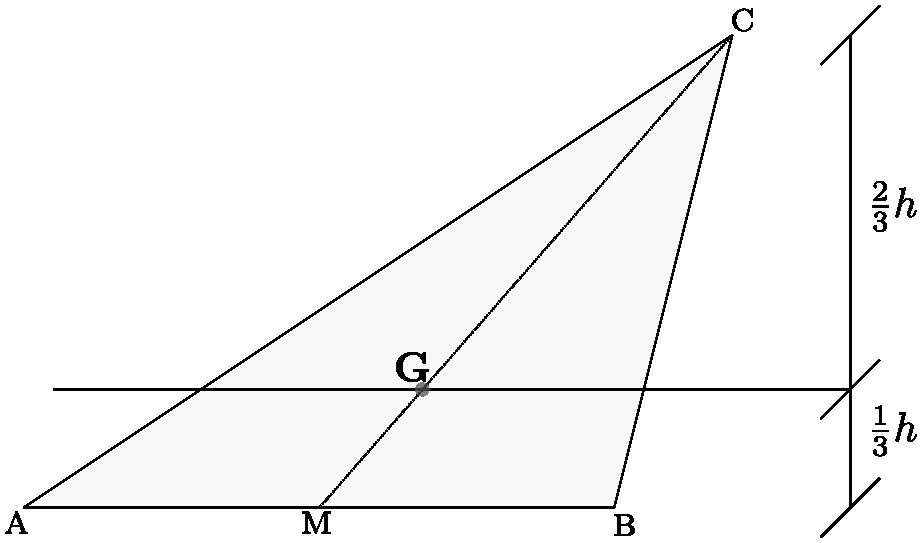
\includegraphics[width=0.5\textwidth]{Immagini/Parte_1/Figura1_6/Figura1_6.pdf}
\caption{}
\label{figura1-6}
\end{figure}
%----------------------------------------------------------------------------------------

\noindent Quest'ultima proposizione consente di individuare il baricentro di numerose figure, tra cui il triangolo (anche scaleno). 

\noindent Con riferimento alla figura~\ref{figura1-6}, la mediana \textsc{cm} è asse di simmetria rispetto alla direzione del lato \textsc{ab}: essa, infatti, dimezza tutti i segmenti interni al triangolo e paralleli al lato \textsc{ab}. 

\noindent Pertanto, in forza della precedente proposizione, il baricentro di un triangolo qualunqe è nelle intersezioni delle tre mediane. E ciò, con semplici considerazione geometriche, porta a concludere che la distanza di $\mathbf{G}$ da ogni lato del triangolo è uguale ad $1/3$ dell'altezza relativa al lato in questione. 
%---------------------------------------------------------------------------------------------------------------------------------------------
\renewcommand{\thefigure}{1~-~7}
\begin{figure}[h]
\centering
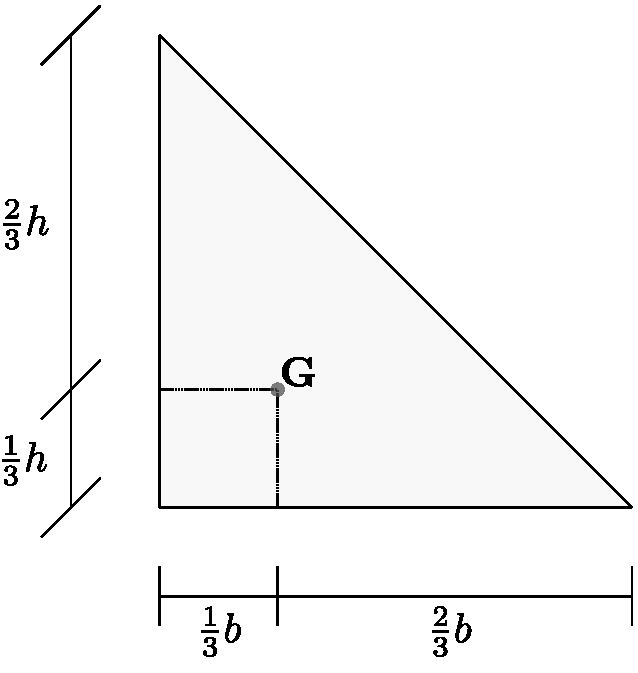
\includegraphics[width=0.45\textwidth]{Immagini/Parte_1/Figura1_7/Figura1_7.pdf}
\caption{}
\label{figura1-7}
\end{figure}
%----------------------------------------------------------------------------------------
\noindent La figura~\ref{figura1-7} illustra il caso del triangolo rettangolo.

\noindent Per determinare il baricentro di una figura piana qualunque si procede così:
%----------------------------------------------------------------------------------------
\begin{enumerate}
\item si assumono due assi di riferimento $x$ ed $y$ scelti a piacere
\item si suddivide la figura in figure parziali (di ognuna delle quali si conosca il baricentro e si sappia calcolare l'area $A_i$)
\item si calcolano $S_{ix}$ ed $S_{iy}$ (momenti statici della generica figura parziale)
\item si calcolano:
\begin{align*}
A    &= \sum_{i=1}^n A_i \\
S_x &= \sum_{i=1}^n S_{ix} \\
S_y &= \sum_{i=1}^n S_{iy}
\end{align*}
\item dalle~\eqref{equazione1-4a} e~\eqref{equazione1-4b} si ricava immediatamente 
%---------------------------------------------------------------------------------------------------------------------------------------------
\begin{align} 
x_G    &= \frac{S_y}{A} \tag{1.5a} \label{equazione1-5a} \\
y_G    &= \frac{S_x}{A} \tag{1.5b} \label{equazione1-5b}
\end{align}
%---------------------------------------------------------------------------------------------------------------------------------------------
\end{enumerate}
%----------------------------------------------------------------------------------------

\noindent Le uguaglianze scritte al punto $4.$ della procedura appena illustrata, sono legittimate dalla ben nota proprietà di additività degli integrali definiti (e tali sono $A$, $S_x$ ed $S_y$).
%----------------------------------------------------------------------------------------
\clearpage
\section{Esercizi}
%----------------------------------------------------------------------------------------
\paragraph{Esercizio 1.1}
%----------------------------------------------------------------------------------------
Determinare il baricentro del profilato illustrato in figura.
%---------------------------------------------------------------------------------------------------------------------------------------------
\renewcommand{\thefigure}{1.1~-~1}
\begin{figure}[h]
\centering
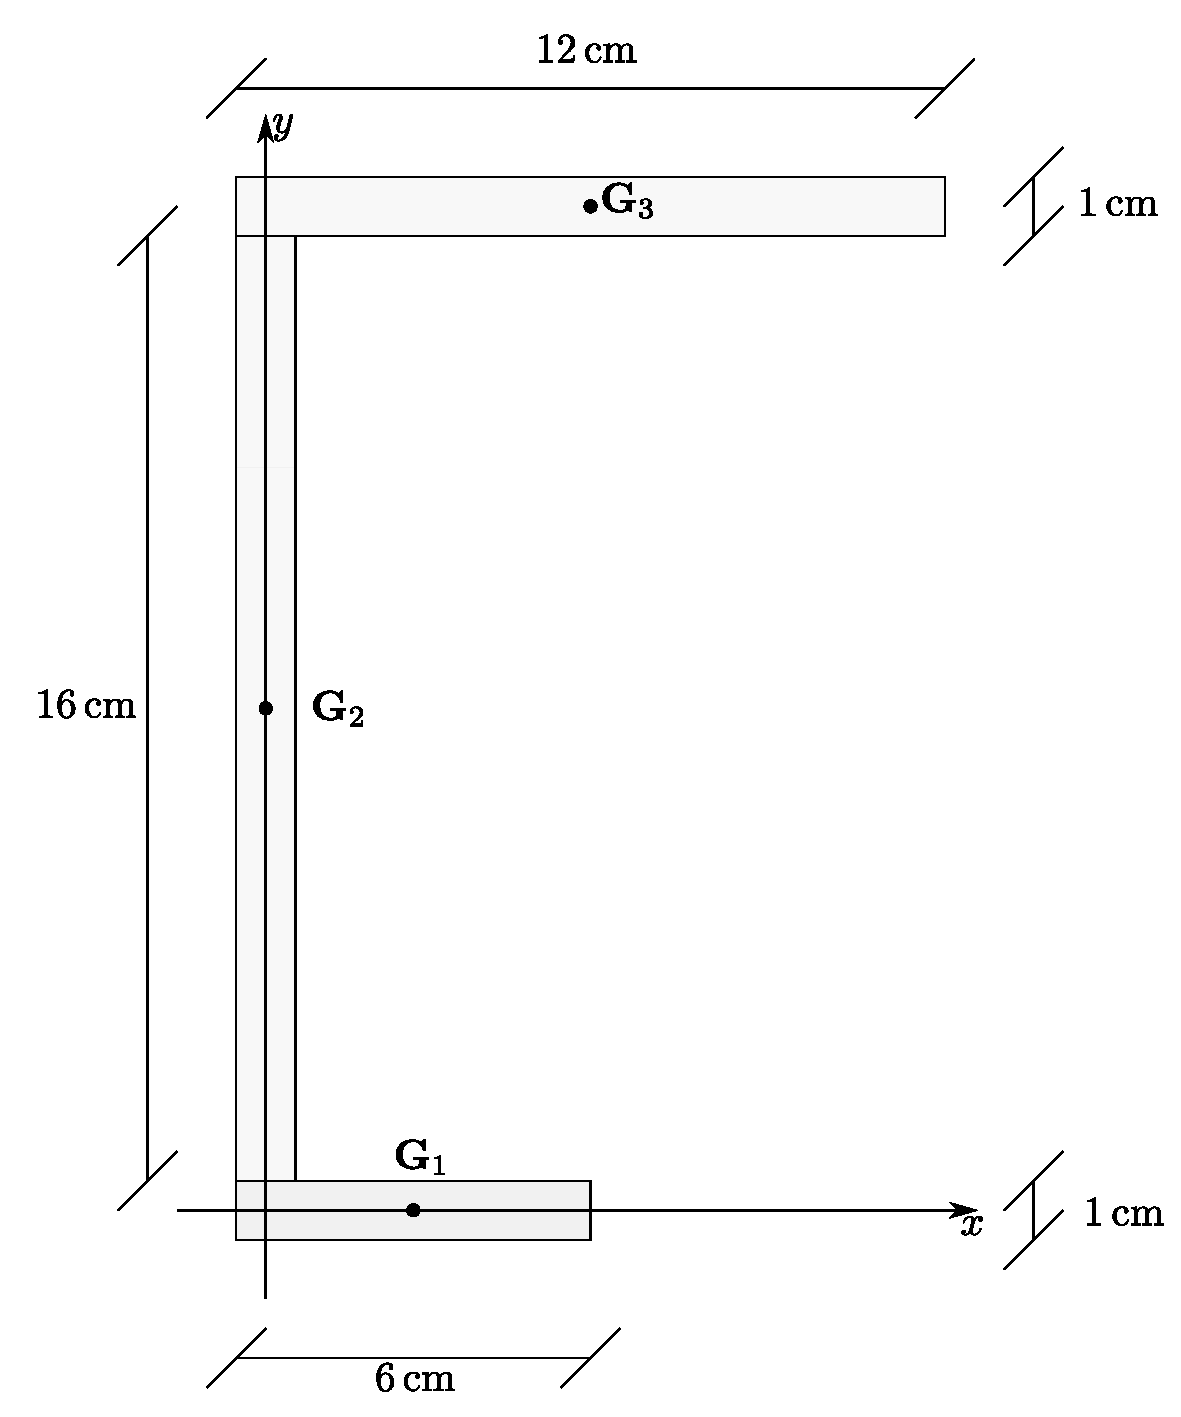
\includegraphics[width=0.80\textwidth]{Immagini/Parte_1/Esercizio1_1/Esercizio1_1.pdf}
\caption{}
\label{Esercizio1_1_1}
\end{figure}
%----------------------------------------------------------------------------------------

\noindent Il profilato è ovviamente interpretabile come unione di $3$ rettangoli (i cui baricentri si sono indicati con $\mathbf{G}_1$, $\mathbf{G}_2$ e $\mathbf{G}_3$). 

\noindent I due assi di riferimento assunti sono certamente quelli che consentono la massima semplificazione nel calcolo dei momenti statici. Risulta dunque:
%----------------------------------------------------------------------------------------
\begin{equation*}
\begin{aligned}
A &= 6\,\textup{cm}^2 \\
A &= 16\,\textup{cm}^2 \\
A &= 12\,\textup{cm}^2
\end{aligned}
\,\,\Biggr\}\,\, A = 34\,\textup{cm}^2
\end{equation*}
%----------------------------------------------------------------------------------------
%----------------------------------------------------------------------------------------
\begin{equation*}
\begin{aligned}
S_{1x} &= 0\,\textup{cm}^3 \\
S_{2x} &= 16\times 8.5 = 136\,\textup{cm}^3 \\
S_{3x} &= 12\times 17  = 204\,\textup{cm}^3
\end{aligned}
\,\,\Biggr\}\,\, S_x = 340\,\textup{cm}^3
\end{equation*}
%----------------------------------------------------------------------------------------
%----------------------------------------------------------------------------------------
\begin{equation*}
\begin{aligned}
S_{1y} &= 6\times 2.5 = 15\,\textup{cm}^3 \\
S_{2y} &= 0\,\textup{cm}^3 \\
S_{3y} &= 12\times 5.5  = 66\,\textup{cm}^3
\end{aligned}
\,\,\Biggr\}\,\, S_y = 81\,\textup{cm}^3
\end{equation*}
%----------------------------------------------------------------------------------------
Pertanto, applicando le equazioni~\eqref{equazione1-5a} e~\eqref{equazione1-5b}:
%---------------------------------------------------------------------------------------------------------------------------------------------
\begin{align*} 
x_G    &= \frac{S_y}{A} = \frac{81}{34} = 2.38\,\textup{cm}  \\
y_G    &= \frac{S_x}{A} = \frac{340}{34} = 10\,\textup{cm}
\end{align*}
%---------------------------------------------------------------------------------------------------------------------------------------------
%---------------------------------------------------------------------------------------------------------------------------------------------
\renewcommand{\thefigure}{1.1~-~2}
\begin{figure}[h]
\centering
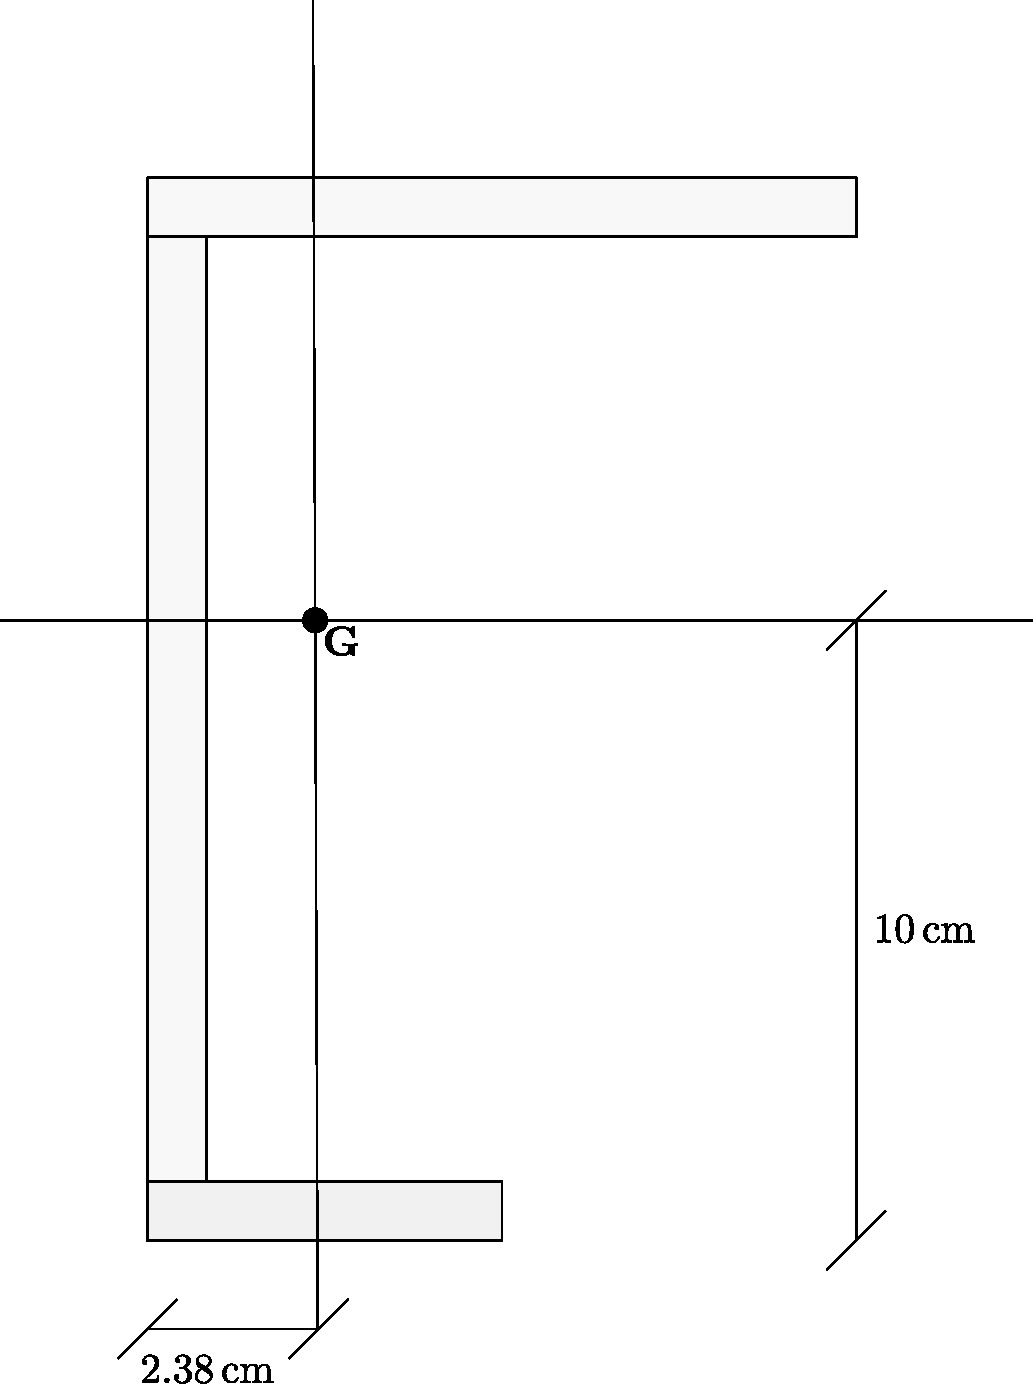
\includegraphics[width=0.45\textwidth]{Immagini/Parte_1/Esercizio1_1/Esercizio1_1_2.pdf}
\caption{}
\label{Esercizio1_1_2}
\end{figure}
%----------------------------------------------------------------------------------------
\paragraph{Esercizio 1.2}
Determinare il baricentro della figura assegnata avendo presente che il cerchio è un foro. 
%---------------------------------------------------------------------------------------------------------------------------------------------
\renewcommand{\thefigure}{1.2~-~1}
\begin{figure}[h]
\centering
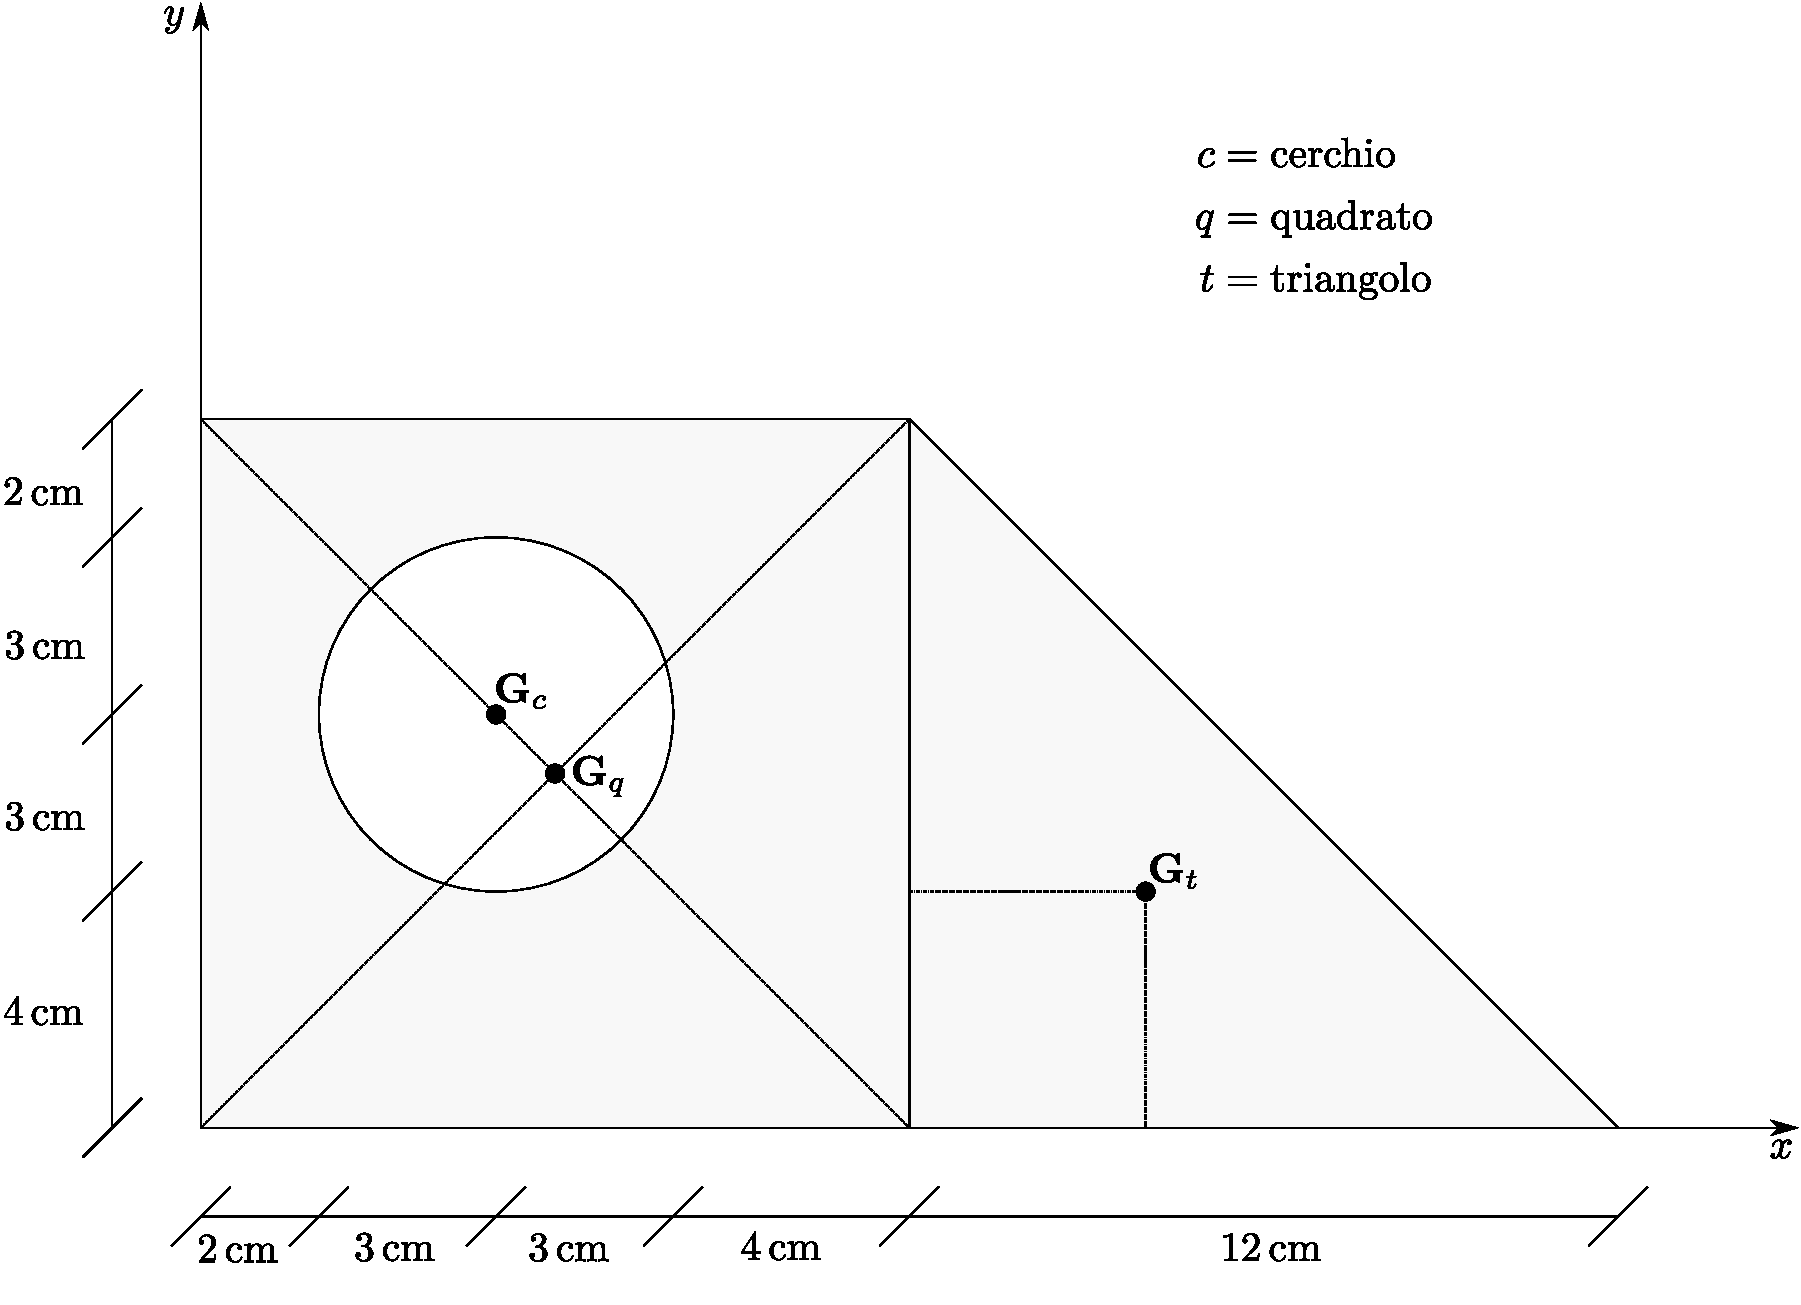
\includegraphics[width=0.89\textwidth]{Immagini/Parte_1/Esercizio1_2/Esercizio1_2_1.pdf}
\caption{}
\label{Esercizio1_2}
\end{figure}
%----------------------------------------------------------------------------------------
%----------------------------------------------------------------------------------------
\begin{equation*}
\begin{aligned}
A_t &= \frac{1}{2}12^2 = 72\,\textup{cm}^2 \\
A_q &= 12^2 = 144\,\textup{cm}^2 \\
A_c &= \pi3^2 = 28.26\,\textup{cm}^2
\end{aligned}
\,\,\Biggr\}\,\, A = 72+144-28.26 = 187.74\,\textup{cm}^2
\end{equation*}
%----------------------------------------------------------------------------------------
%----------------------------------------------------------------------------------------
\begin{equation*}
\begin{aligned}
S_{\textup{t}x} &= 72\times 4 = 288\,\textup{cm}^3 \\
S_{\textup{q}x} &= 144\times 6 = 864\,\textup{cm}^3 \\
S_{\textup{c}x} &= 28.26\times 17  = 480.42\,\textup{cm}^3
\end{aligned}
\,\,\Biggr\}\,\, S_x = 288+864-480.42 = 671.58\,\textup{cm}^3
\end{equation*}
%----------------------------------------------------------------------------------------
%----------------------------------------------------------------------------------------
\begin{equation*}
\begin{aligned}
S_{\textup{t}y} &= 72\times 16 = 1152\,\textup{cm}^3 \\
S_{\textup{q}y} &= 144\times 6 = 864\,\textup{cm}^3 \\
S_{\textup{c}y} &= 28.26\times 5  = 141.30\,\textup{cm}^3
\end{aligned}
\,\,\Biggr\}\,\, S_y = 1152+864-141.30 = 1874.70\,\textup{cm}^3
\end{equation*}
%----------------------------------------------------------------------------------------
%---------------------------------------------------------------------------------------------------------------------------------------------
\begin{align*} 
x_G    &= \frac{S_y}{A} = \frac{1874.70}{187.74} = 9.986\,\textup{cm}  \\
y_G    &= \frac{S_x}{A} = \frac{951.31}{187.74} = 5.067\,\textup{cm}
\end{align*}
%---------------------------------------------------------------------------------------------------------------------------------------------
\paragraph{Esercizio 1.3}
Formulare i momenti statici e la posizione del baricentro per il settore di corona circolare rappresentato in figura.
%---------------------------------------------------------------------------------------------------------------------------------------------
\renewcommand{\thefigure}{1.3~-~1}
\begin{figure}[ht]
\centering
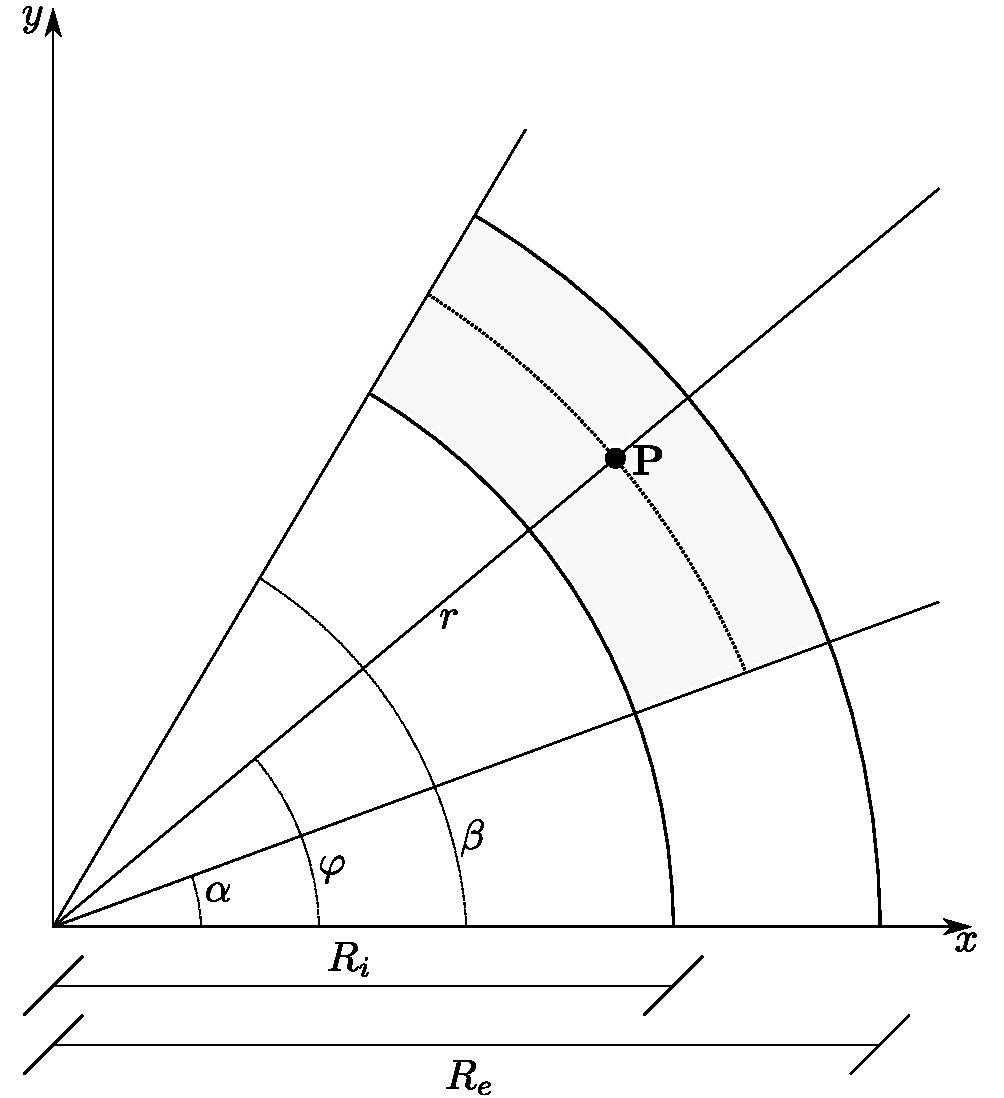
\includegraphics[width=0.8\textwidth]{Immagini/Parte_1/Esercizio1_3/Esercizio1_3.pdf}
\caption{}
\label{Esercizio1_3}
\end{figure}
%----------------------------------------------------------------------------------------

\noindent Sappiamo che 
%----------------------------------------------------------------------------------------
\begin{equation*}
A = \frac{\beta-\alpha}{2}(R_e^2-R_i^2)
\end{equation*}
%----------------------------------------------------------------------------------------
Per conoscere $S_x$ ed $S_y$ dobbiamo calcolare gli integrali: 
%----------------------------------------------------------------------------------------
\begin{align*}
S_x &= \int\int_A ydA \\
S_y &= \int\int_A xdA
\end{align*}
%----------------------------------------------------------------------------------------
Naturalmente conviene introdurre le coordinate polari: 
%----------------------------------------------------------------------------------------
\begin{equation*}
\,\,\Biggr\{\,\, 
\begin{aligned}
x &= r\cos\varphi \\
y &= r\sin\varphi
\end{aligned}
\end{equation*}
%----------------------------------------------------------------------------------------
Lo \emph{Jacobiano} della trasformazione $(x,\,y)\,\leftrightarrow\,(r,\,\varphi)$ vale: 
%----------------------------------------------------------------------------------------
\begin{equation*}
\lvert \, J \, \lvert =
\begin{vmatrix}
\frac{\partial x}{\partial r} & \frac{\partial y}{\partial r}\\
\frac{\partial x}{\partial\varphi} & \frac{\partial y}{\partial\varphi}
\end{vmatrix}
=
\begin{vmatrix}
\cos\varphi & \sin\varphi \\
-r\sin\varphi & r\cos\varphi
\end{vmatrix}
= r
\end{equation*}
%----------------------------------------------------------------------------------------
E dunque
%----------------------------------------------------------------------------------------
\begin{align*}
S_x &= \int\int_A ydxdy = \int\int_A r\sin\varphi rdrd\varphi = \int_{R_{i}}^{R_{e}} r^2dr\int_\alpha^\beta \sin\varphi d\varphi = \frac{1}{3}(R_e^3-R_i^3)(\cos\alpha-\cos\beta) \\
S_y &= \int\int_A xdxdy = \int\int_A r\cos\varphi rdrd\varphi = \int_{R_{i}}^{R_{e}} r^2dr\int_\alpha^\beta \cos\varphi d\varphi = \frac{1}{3}(R_e^3-R_i^3)(\sin\beta-\sin\alpha) 
\end{align*} 
%----------------------------------------------------------------------------------------
Le coordinate del baricentro sono, pertanto: 
%---------------------------------------------------------------------------------------------------------------------------------------------
\begin{align*} 
x_G    &= \frac{S_y}{A} = \frac{2}{3} \frac{(R_e^3-R_i^3)}{(R_e^2-R_i^2)}\frac{(\sin\beta-\sin\alpha)}{\beta-\alpha}  \\
y_G    &= \frac{S_x}{A} = \frac{2}{3} \frac{(R_e^3-R_i^3)}{(R_e^2-R_i^2)}\frac{(\cos\alpha-\cos\beta)}{\beta-\alpha}
\end{align*}
%---------------------------------------------------------------------------------------------------------------------------------------------
Vale la pena di sottolineare che il settore di corona circolare ha un asse di simmetria ortogonale; il baricentro, ovviamente, sta su tale asse e la sua distanza dal centro (che è l'origine del riferimento) è ovviamente:%---------------------------------------------------------------------------------------------------------------------------------------------
\begin{equation*}
d_G = \sqrt{x_G^2+y_G^2}
\end{equation*}
%---------------------------------------------------------------------------------------------------------------------------------------------
Utilizzando le precedenti formulazioni di $x_G$ ed $y_G$ con semplici passaggi si trova:
%---------------------------------------------------------------------------------------------------------------------------------------------
\begin{equation*}
d_G = \frac{2}{3}\frac{(R_e^3-R_i^3)}{(R_e^2-R_i^2)}\frac{\sin\frac{\beta-\alpha}{2}}{\frac{\beta-\alpha}{2}}
\end{equation*}
%---------------------------------------------------------------------------------------------------------------------------------------------
\clearpage
%---------------------------------------------------------------------------------------------------------------------------------------------
\paragraph{Esercizio 1.4}
Determinare il baricentro del quarto di cerchio rappresentato in figura e calcolarne $S_x$ ed $S_y$.
%---------------------------------------------------------------------------------------------------------------------------------------------
\renewcommand{\thefigure}{1.4~-~1}
\begin{figure}[ht]
\centering
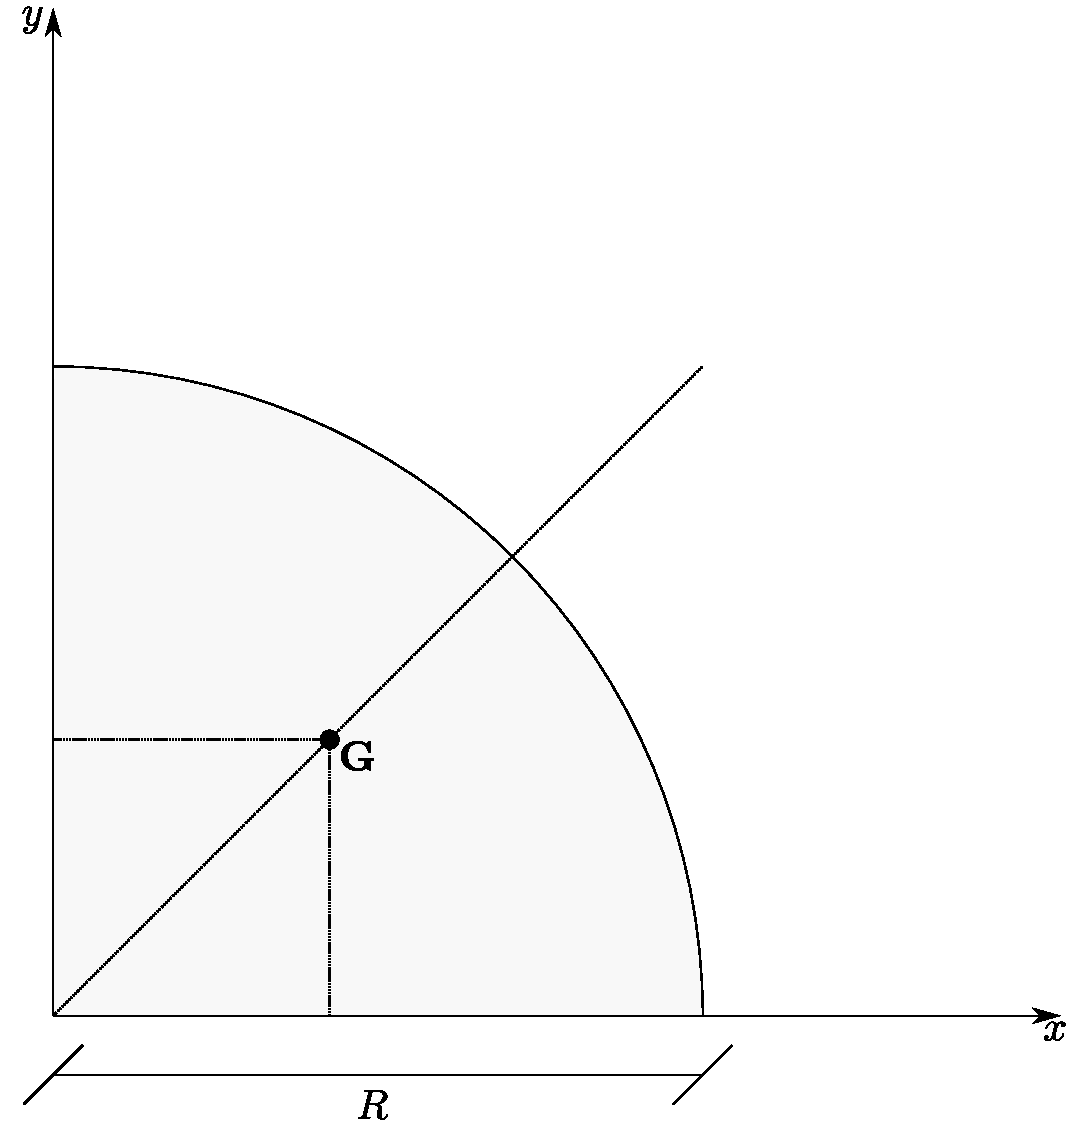
\includegraphics[width=0.6\textwidth]{Immagini/Parte_1/Esercizio1_4/Esercizio1_4.pdf}
\caption{}
\label{Esercizio1_4}
\end{figure}
%----------------------------------------------------------------------------------------
Per calcolare la distanza del baricentro dal centro possiamo applicare la formula per $d_G$ trovata nell'esercizio precedente, ponendo in essa: 
%----------------------------------------------------------------------------------------
\begin{align*}
R_e &= R \\ 
R_i &= 0 \\
\alpha &= 0 \\ 
\beta &=\frac{\pi}{2}
\end{align*}
%----------------------------------------------------------------------------------------
E così si trova: 
%----------------------------------------------------------------------------------------
\begin{equation*}
\lvert \, \textup{OG} \, \lvert = \frac{2}{3}R\frac{\sin\frac{\pi}{4}}{\frac{\pi}{4}} = \frac{4\sqrt{2}}{3\pi}R = 0.6R 
\end{equation*}
%----------------------------------------------------------------------------------------
Le coordinate del baricentro $\mathbf{G}$ sono, ovviamente: 
%----------------------------------------------------------------------------------------
\begin{equation*}
x_G = y_G = \frac{\sqrt{2}}{2}d_G = \frac{4}{3\pi}R = 0.4244R
\end{equation*}
%----------------------------------------------------------------------------------------
Naturalmente, risulta:
%----------------------------------------------------------------------------------------
\begin{equation*}
S_x = S_y = A\times x_G = \frac{\pi}{4}R^2\frac{4}{3\pi}R = \frac{1}{3}R^3
\end{equation*}
%----------------------------------------------------------------------------------------
\paragraph{Esercizio 1.5}
%----------------------------------------------------------------------------------------
Determinare il baricentro del semicerchio rappresentato in figura e calcolarne $S_x$ ed $S_y$. 
%----------------------------------------------------------------------------------------
%---------------------------------------------------------------------------------------------------------------------------------------------
\renewcommand{\thefigure}{1.5~-~1}
\begin{figure}[ht]
\centering
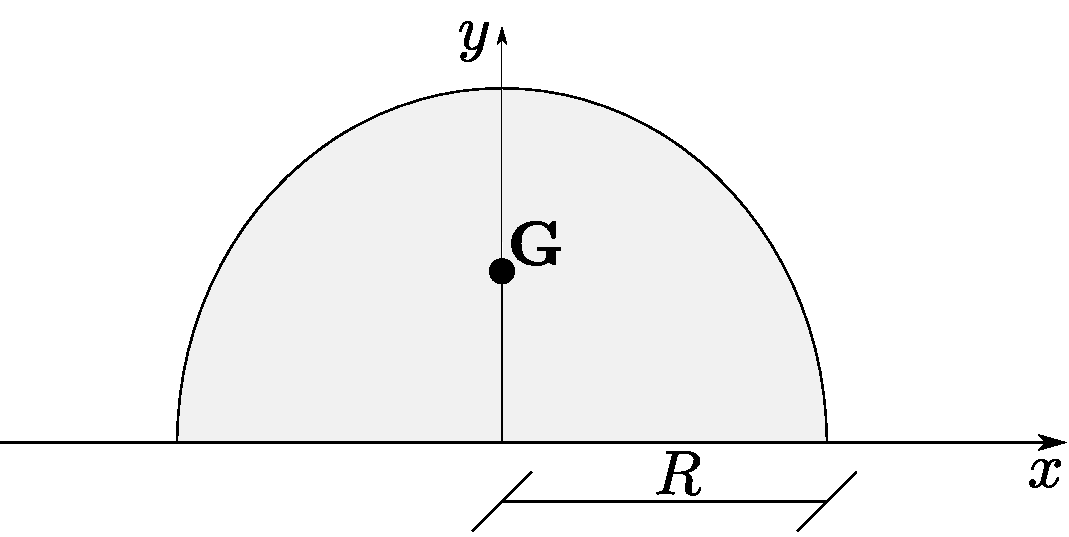
\includegraphics[width=\textwidth]{Immagini/Parte_1/Esercizio1_5/Esercizio1_5.pdf}
\caption{}
\label{Esercizio1_5}
\end{figure}
%----------------------------------------------------------------------------------------

\noindent Sarà ovviamente 
%----------------------------------------------------------------------------------------
\begin{align*}
x_G &= 0 \\ 
S_y &= 0
\end{align*}
%----------------------------------------------------------------------------------------
Per calcolare $y_G$ possiamo utilizzare la formula ricavata nell'Esercizio 1.3 ponendo in essa: 
%----------------------------------------------------------------------------------------
\begin{align*}
R_e &= R \\ 
R_i &= 0 \\
\alpha &=0 \\ 
\beta &=\pi
\end{align*}
%----------------------------------------------------------------------------------------
E così si trova:
%----------------------------------------------------------------------------------------
\begin{equation*}
y_G = \frac{2}{3}R\frac{\cos 0 - \cos\pi}{\pi-0} = \frac{4}{3\pi}R \approx 0.4244R
\end{equation*}
%----------------------------------------------------------------------------------------
Com'era lecito attendersi, $y_G$ è uguale a quella relativa ad un quarto di cerchio. Ovviamente: 
%----------------------------------------------------------------------------------------
\begin{equation*}
S_x = A\times y_G = \frac{\pi}{2}R^2\frac{4}{3\pi}R = \frac{2}{3}R
\end{equation*}
%----------------------------------------------------------------------------------------
\clearpage
\paragraph{Esercizio 1.6}
%----------------------------------------------------------------------------------------
Determinare il baricentro della zona ombreggiata rappresentata in figura. 
%---------------------------------------------------------------------------------------------------------------------------------------------
\renewcommand{\thefigure}{1.6~-~1}
\begin{figure}[h]
\centering
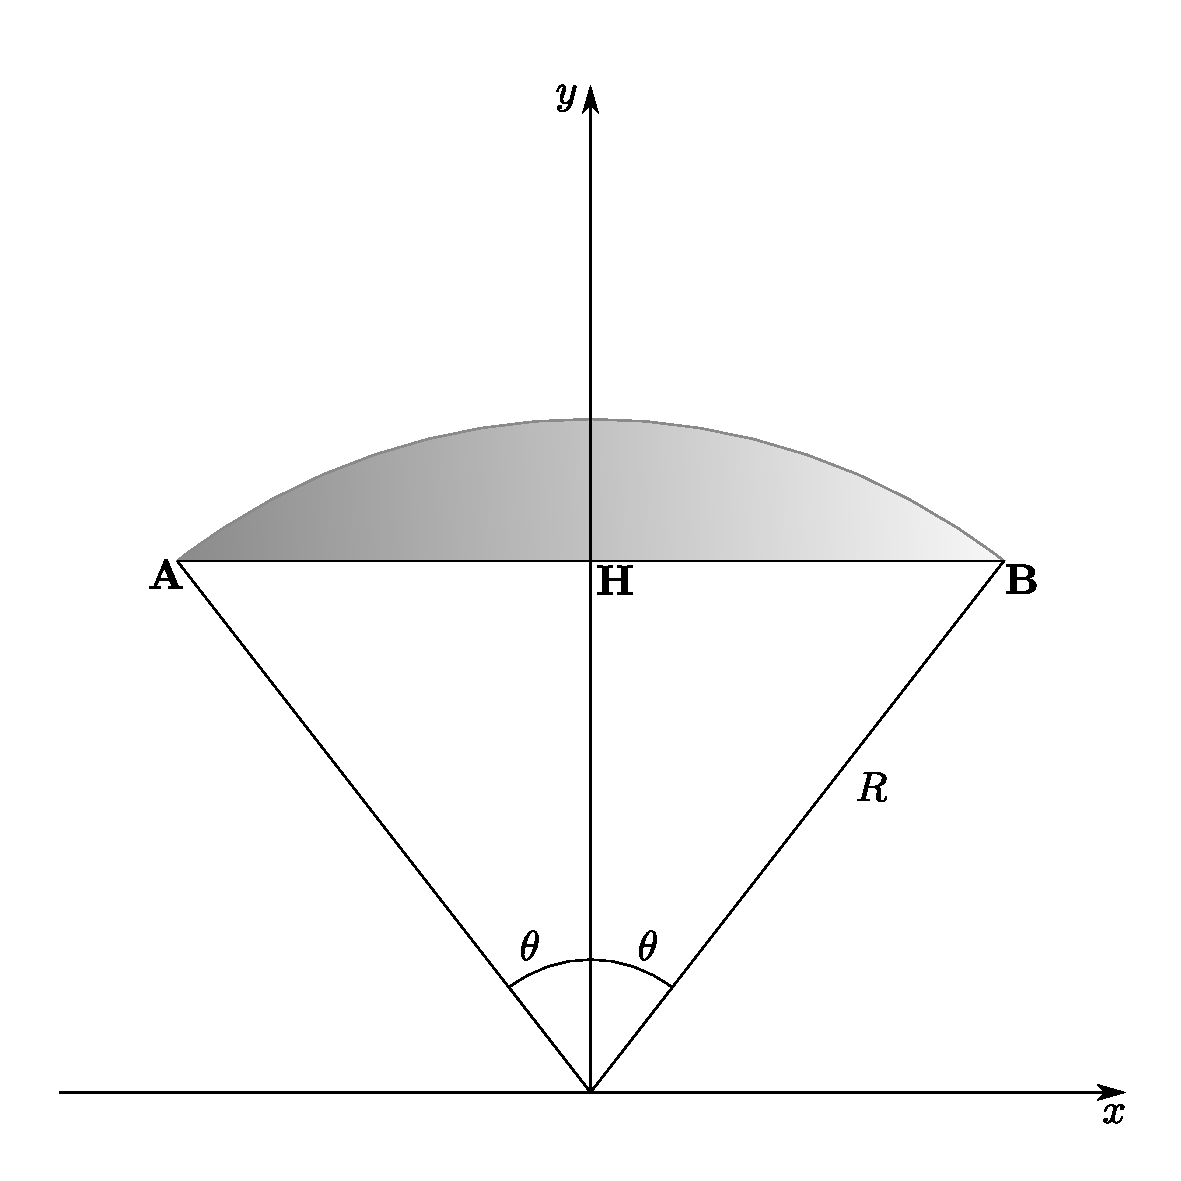
\includegraphics[width=0.75\textwidth]{Immagini/Parte_1/Esercizio1_6/Esercizio1_6.pdf}
\caption{}
\label{Esercizio1_6}
\end{figure}
%----------------------------------------------------------------------------------------

\noindent È evidente che $x_G=0$. Per calcolare $y_G$ ci servono $S_x$ ed $A$; sia $S_x$ che $A$ possono calcolarsi per differenza: 
%----------------------------------------------------------------------------------------
\begin{align*}
A &= \textup{Area settore ombreggiato} - \textup{Area triangolo} = A_s - A_t \\
S_x &= S_{\textup{s}x} - S_{\textup{t}x}
\end{align*}
%----------------------------------------------------------------------------------------
Dalla figura si ha: 
%----------------------------------------------------------------------------------------
\begin{align*}
A_s &= \theta R^2 \\ 
A_t &= \frac{1}{2}\, \lvert \, \textup{AB} \, \lvert \, \lvert \, \textup{OH} \, \lvert = R^2 \sin\theta\cos\theta
\end{align*}
%----------------------------------------------------------------------------------------
da cui 
%----------------------------------------------------------------------------------------
\begin{equation*}
A = (\theta-\sin\theta\cos\theta)R^2
\end{equation*}
%----------------------------------------------------------------------------------------
Per calcolare $S_{\textup{s}x}$ possiamo utilizzare la formula ricavata nell'esercizio 1.3 ponendo in essa:
%----------------------------------------------------------------------------------------
\begin{align*}
R_e &= R \\
R_i &= 0 \\
\alpha &= \frac{\pi}{2}-\theta \\ 
\beta &= \frac{\pi}{2}+\theta
\end{align*}
%----------------------------------------------------------------------------------------
E così si trova:
%----------------------------------------------------------------------------------------
\begin{align*}
S_{\textup{s}x} &= \frac{1}{3}\Biggr[\cos\biggl(\frac{\pi}{2}-\theta\biggr)-\cos\biggl(\frac{\pi}{2}+\theta\biggr)\Biggl]=\frac{2}{3}R^3 \sin\theta \\
S_{\textup{t}x} &= \frac{2}{3}A_t\, \lvert \, \textup{OH} \, \lvert =R^2 \sin\theta\cos\theta\frac{2}{3}R\cos\theta =\frac{2}{3}R^3 \sin\theta\cos^{2}\theta
\end{align*}
%----------------------------------------------------------------------------------------
Quindi:
%----------------------------------------------------------------------------------------
\begin{equation*}
S_x = S_{\textup{s}x}-S_{\textup{t}x} = \frac{2}{3}R^3 \sin\theta - \frac{2}{3}R^3 \sin\theta\cos^{2}\theta = \frac{2}{3}R^3 \sin^{3}\theta
\end{equation*}
%----------------------------------------------------------------------------------------
In definitiva:
%----------------------------------------------------------------------------------------
\begin{equation*}
y_G = \frac{S_x}{A} = \frac{2}{3}R^{3}\sin^{3}\theta\frac{1}{R^{2}(\theta-\sin\theta\cos\theta)}
\end{equation*}
%----------------------------------------------------------------------------------------
e semplificando
%----------------------------------------------------------------------------------------
\begin{equation*}
y_G = \frac{S_x}{A} = \frac{2}{3}R\frac{\sin^{3}\theta}{(\theta-\sin\theta\cos\theta)}
\end{equation*}
%----------------------------------------------------------------------------------------
\clearpage
\paragraph{Esercizio 1.7}
%----------------------------------------------------------------------------------------
Formulare i momenti statici e la posizione del baricentro per il settore di corona circolare (di spessore molto sottile) rappresentato in figura. 
%---------------------------------------------------------------------------------------------------------------------------------------------
\renewcommand{\thefigure}{1.7~-~1}
\begin{figure}[h]
\centering
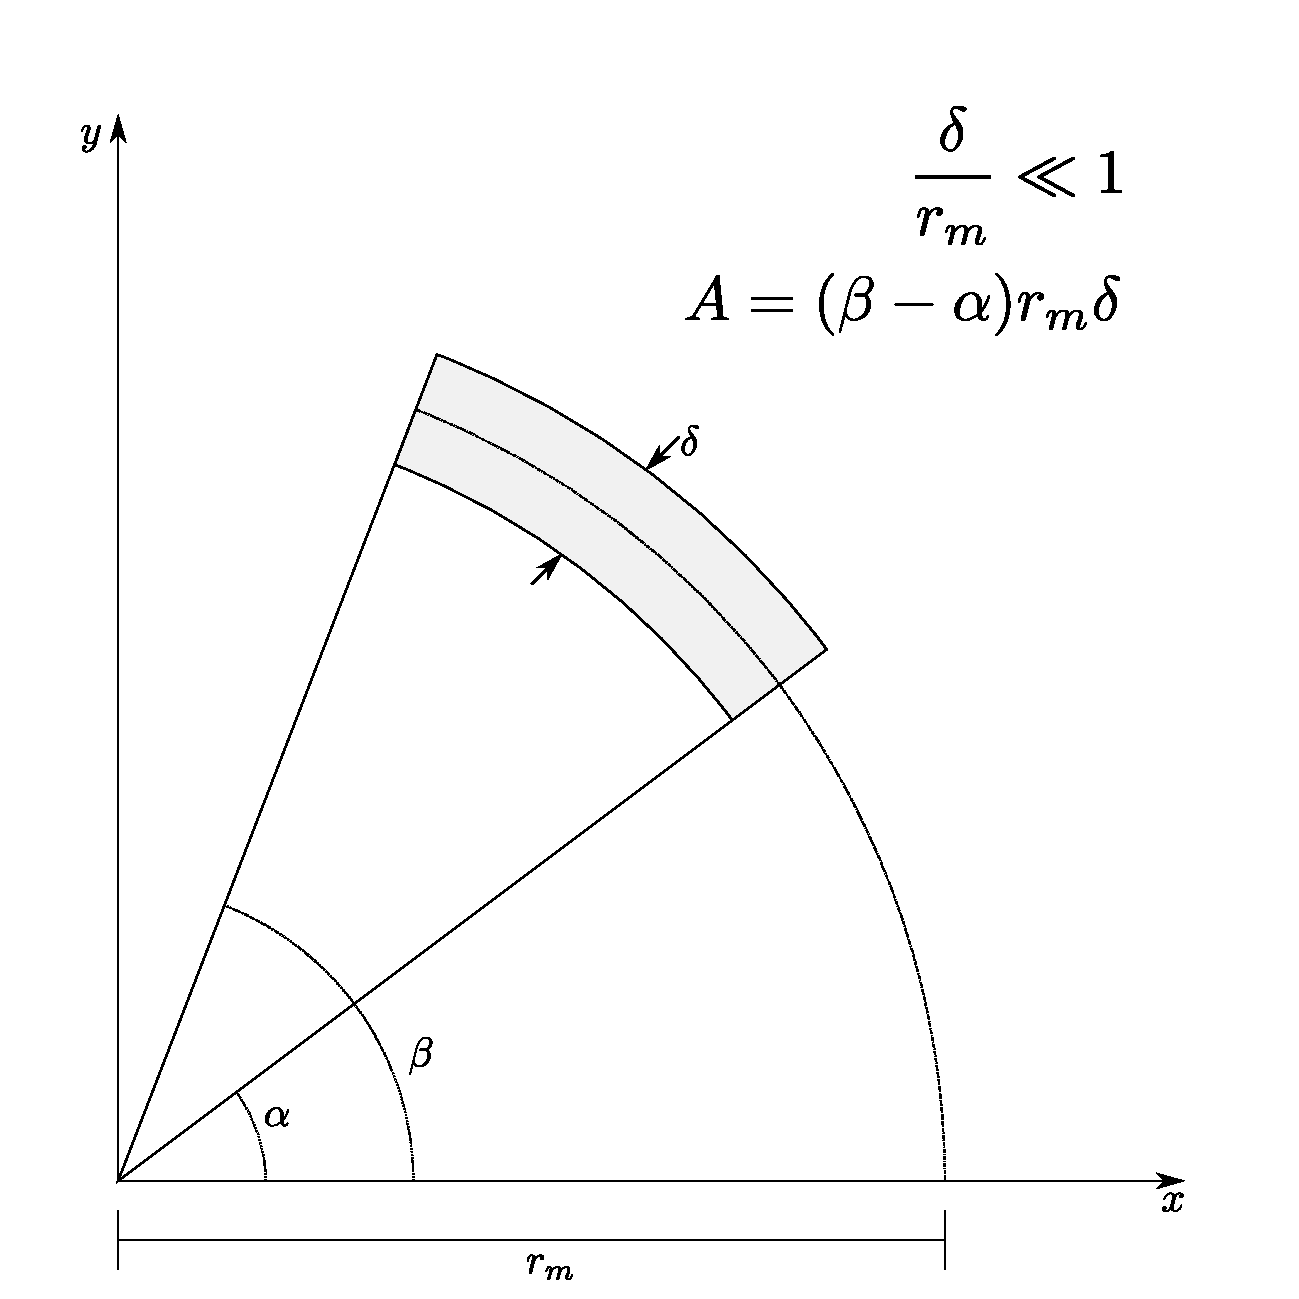
\includegraphics[width=0.75\textwidth]{Immagini/Parte_1/Esercizio1_7/Esercizio1_7.pdf}
\caption{}
\label{Esercizio1_7}
\end{figure}
%----------------------------------------------------------------------------------------

\noindent Possiamo utilizzare i risultati ottenuti nell'Esercizio 1.3 ponendo:
%----------------------------------------------------------------------------------------
\begin{align*}
R_e &= r_m+\frac{\delta}{2} \\
R_i &= r_m-\frac{\delta}{2}
\end{align*}
%----------------------------------------------------------------------------------------
Con semplici calcoli si trova:
%----------------------------------------------------------------------------------------
%----------------------------------------------------------------------------------------
\begin{align*}
R_e^2-R_i^2 &= 2r_m\delta \\
R_e^3-R_i^3 &= \frac{1}{4}(\delta^2+12r_m^2)\delta
\end{align*}
%----------------------------------------------------------------------------------------
e così le formule dell'Esercizio 1.3 divengono:
%----------------------------------------------------------------------------------------
%----------------------------------------------------------------------------------------
\begin{align*}
S_x &= \frac{1}{12}(\delta^2+12r_m^2)(\cos\alpha-\cos\beta)\delta \\
S_y &= \frac{1}{12}(\delta^2+12r_m^2)(\sin\beta-\sin\alpha)\delta
\end{align*}
%----------------------------------------------------------------------------------------
%----------------------------------------------------------------------------------------
\begin{align*}
x_G &= \frac{2}{3}\frac{\frac{1}{4}(\delta^2+12r_m^2)\delta}{2r_m\delta}\frac{\sin\beta-\sin\alpha}{\beta-\alpha} = \frac{1}{12}\frac{\delta^2+12r_m^2}{r_m}\frac{\sin\beta-\sin\alpha}{\beta-\alpha} \\
y_G &= \frac{1}{12}\frac{\delta^2+12r_m^2}{r_m}\frac{\cos\alpha-\cos\beta}{\beta-\alpha}
\end{align*}
%----------------------------------------------------------------------------------------
\begin{equation*}
d_G = \frac{1}{12}\frac{(\delta^2+12r_m^2)}{r_m}\frac{\sin\frac{\beta-\alpha}{2}}{\frac{\beta-\alpha}{2}}
\end{equation*}
%----------------------------------------------------------------------------------------
Tuttavia, se $\frac{\delta}{r_m}\ll1$, è lecito adottare le formule:
%----------------------------------------------------------------------------------------
\begin{align*}
S_x &= r_m^2(\cos\alpha-\cos\beta)\delta \\
S_y &= r_m^2(\sin\beta-\sin\alpha)\delta \\ 
x_G &= r_m\frac{\sin\beta-\sin\alpha}{\beta-\alpha} \\
y_G &= r_m\frac{\cos\alpha-\cos\beta}{\beta-\alpha} \\
d_G &= r_m\frac{\sin\frac{\beta-\alpha}{2}}{\frac{\beta-\alpha}{2}}
\end{align*}
%----------------------------------------------------------------------------------------
nelle quali si è trascurato $\delta^2$ rispetto a $12r_m^3$. 
%----------------------------------------------------------------------------------------

\noindent Vale la pena sottolineare che, nel caso $\frac{\delta}{r_m} = \frac{1}{10}$, l'errore insito nelle suddette formule è pari a:
%----------------------------------------------------------------------------------------
\begin{equation*}
\textup{\textsc{errore}} = \frac{\textup{\textsc{valore esatto}}-\textup{\textsc{valore approssimato}}}{\textup{\textsc{valore esatto}}}
\end{equation*}
%----------------------------------------------------------------------------------------
Quindi: 
%----------------------------------------------------------------------------------------
\begin{equation*}
\epsilon = \frac{\delta^2+12r_m^2-12r_m^2}{\delta^2+12r_m^2} = \frac{1}{1+12\bigl(\frac{r_m}{\delta}\bigr)^2} = \frac{1}{1201} = 0.0008 = 0.08\%
\end{equation*}
%----------------------------------------------------------------------------------------
che, per un ingegnere, \textbf{non è un errore}.